\section{Process definition}
\label{sec:process_definition}

Framed in the context of an intracellular infection which ultimately causes the
host cell to burst, our chosen version of the birth--death--catastrophe model
is constructed in the following way. $\xt$ is a stochastic process of discrete
state space, evaluated in continuous time. It satisfies the Markov property
with transition probabilities dependent only on its current state:
\begin{align*}
\pr{\xx_{t+\Delta t} - \xt = 1} &= \lambda \xt \cdot \delt&&\text{(birth)}\\
\pr{\xx_{t+\Delta t} - \xt = -1} &= \mu \xt  \cdot \delt&&\text{(death)}\\
\pr{\xx_{t+\Delta t} - \xt = 0} &=1 -  (\lambda+\mu+\delta) \xt  \cdot \delt&&\text{(no event)}\\
\pr{\xx_{t+\Delta t} = H} &=\delta \xt  \cdot \delt&&\text{(catastrophe)}
\end{align*}
The count $\xt$ is a number of replicative units, which in our application
represent infectious particles. With rate $\lambda$, a given one of these units
will undergo division, a birth event; with rate $\mu$, a death event. And with
rate $\delta$, a given particle will trigger the catastrophe event. With this
staged as rupture of the infected macrophage, all $\xt$ of the virions or
bacteria are released into the extracellular matrix.

In a duration $\delt$, the probability of a birth occurring is
$\lambda \delt \cdot \xt$: the likelihood of a single unit dividing, multiplied
by the number of units $\xt$. The model is evaluated in the limit
$\delt \to 0$. This is why the above transition probabilities account for only
the occurrence of single events; the likelihood that two or more transitions
occur in $\delt$ time is proportional to $o(\delt)$, and thus vanishes in the
limit.

\figureflag{F3.1}{Process transition diagram}{%
\textbf{Purpose:} the definition of the process at a glance --- the states, the
three transition types, and the two absorbing states, in one schematic.
\textbf{Type:} TikZ schematic, inline with chapter fonts. \textbf{Content:}
states $0,1,2,\ldots,H$ arranged in a horizontal row, each in a rounded box
except $H$, which is drawn as an ellipse to mark its special role; rightward
arrows $n\to n+1$ labelled $\lambda n$; leftward arrows $n\to n-1$ labelled
$\mu n$; long curved arrows from each $n\ge1$ to $H$ labelled $\delta n$; mark
$0$ and $H$ as absorbing (no outgoing arrows, e.g.\ a small filled dot or
``absorbing'' annotation). Optionally fade the middle states with $\cdots$
between $2$ and a generic $n$. \textbf{Labels:} state labels $0,1,2,\dots,H$;
rate labels $\lambda n$, $\mu n$, $\delta n$. \textbf{Style:} TikZ, inline with
chapter fonts, black arrows, rate labels in math mode. \textbf{Placement:}
\Secref{sec:process_definition}, as the first figure of the section, directly
after the transition-probability display.}

\begin{figure}[H]
\centering
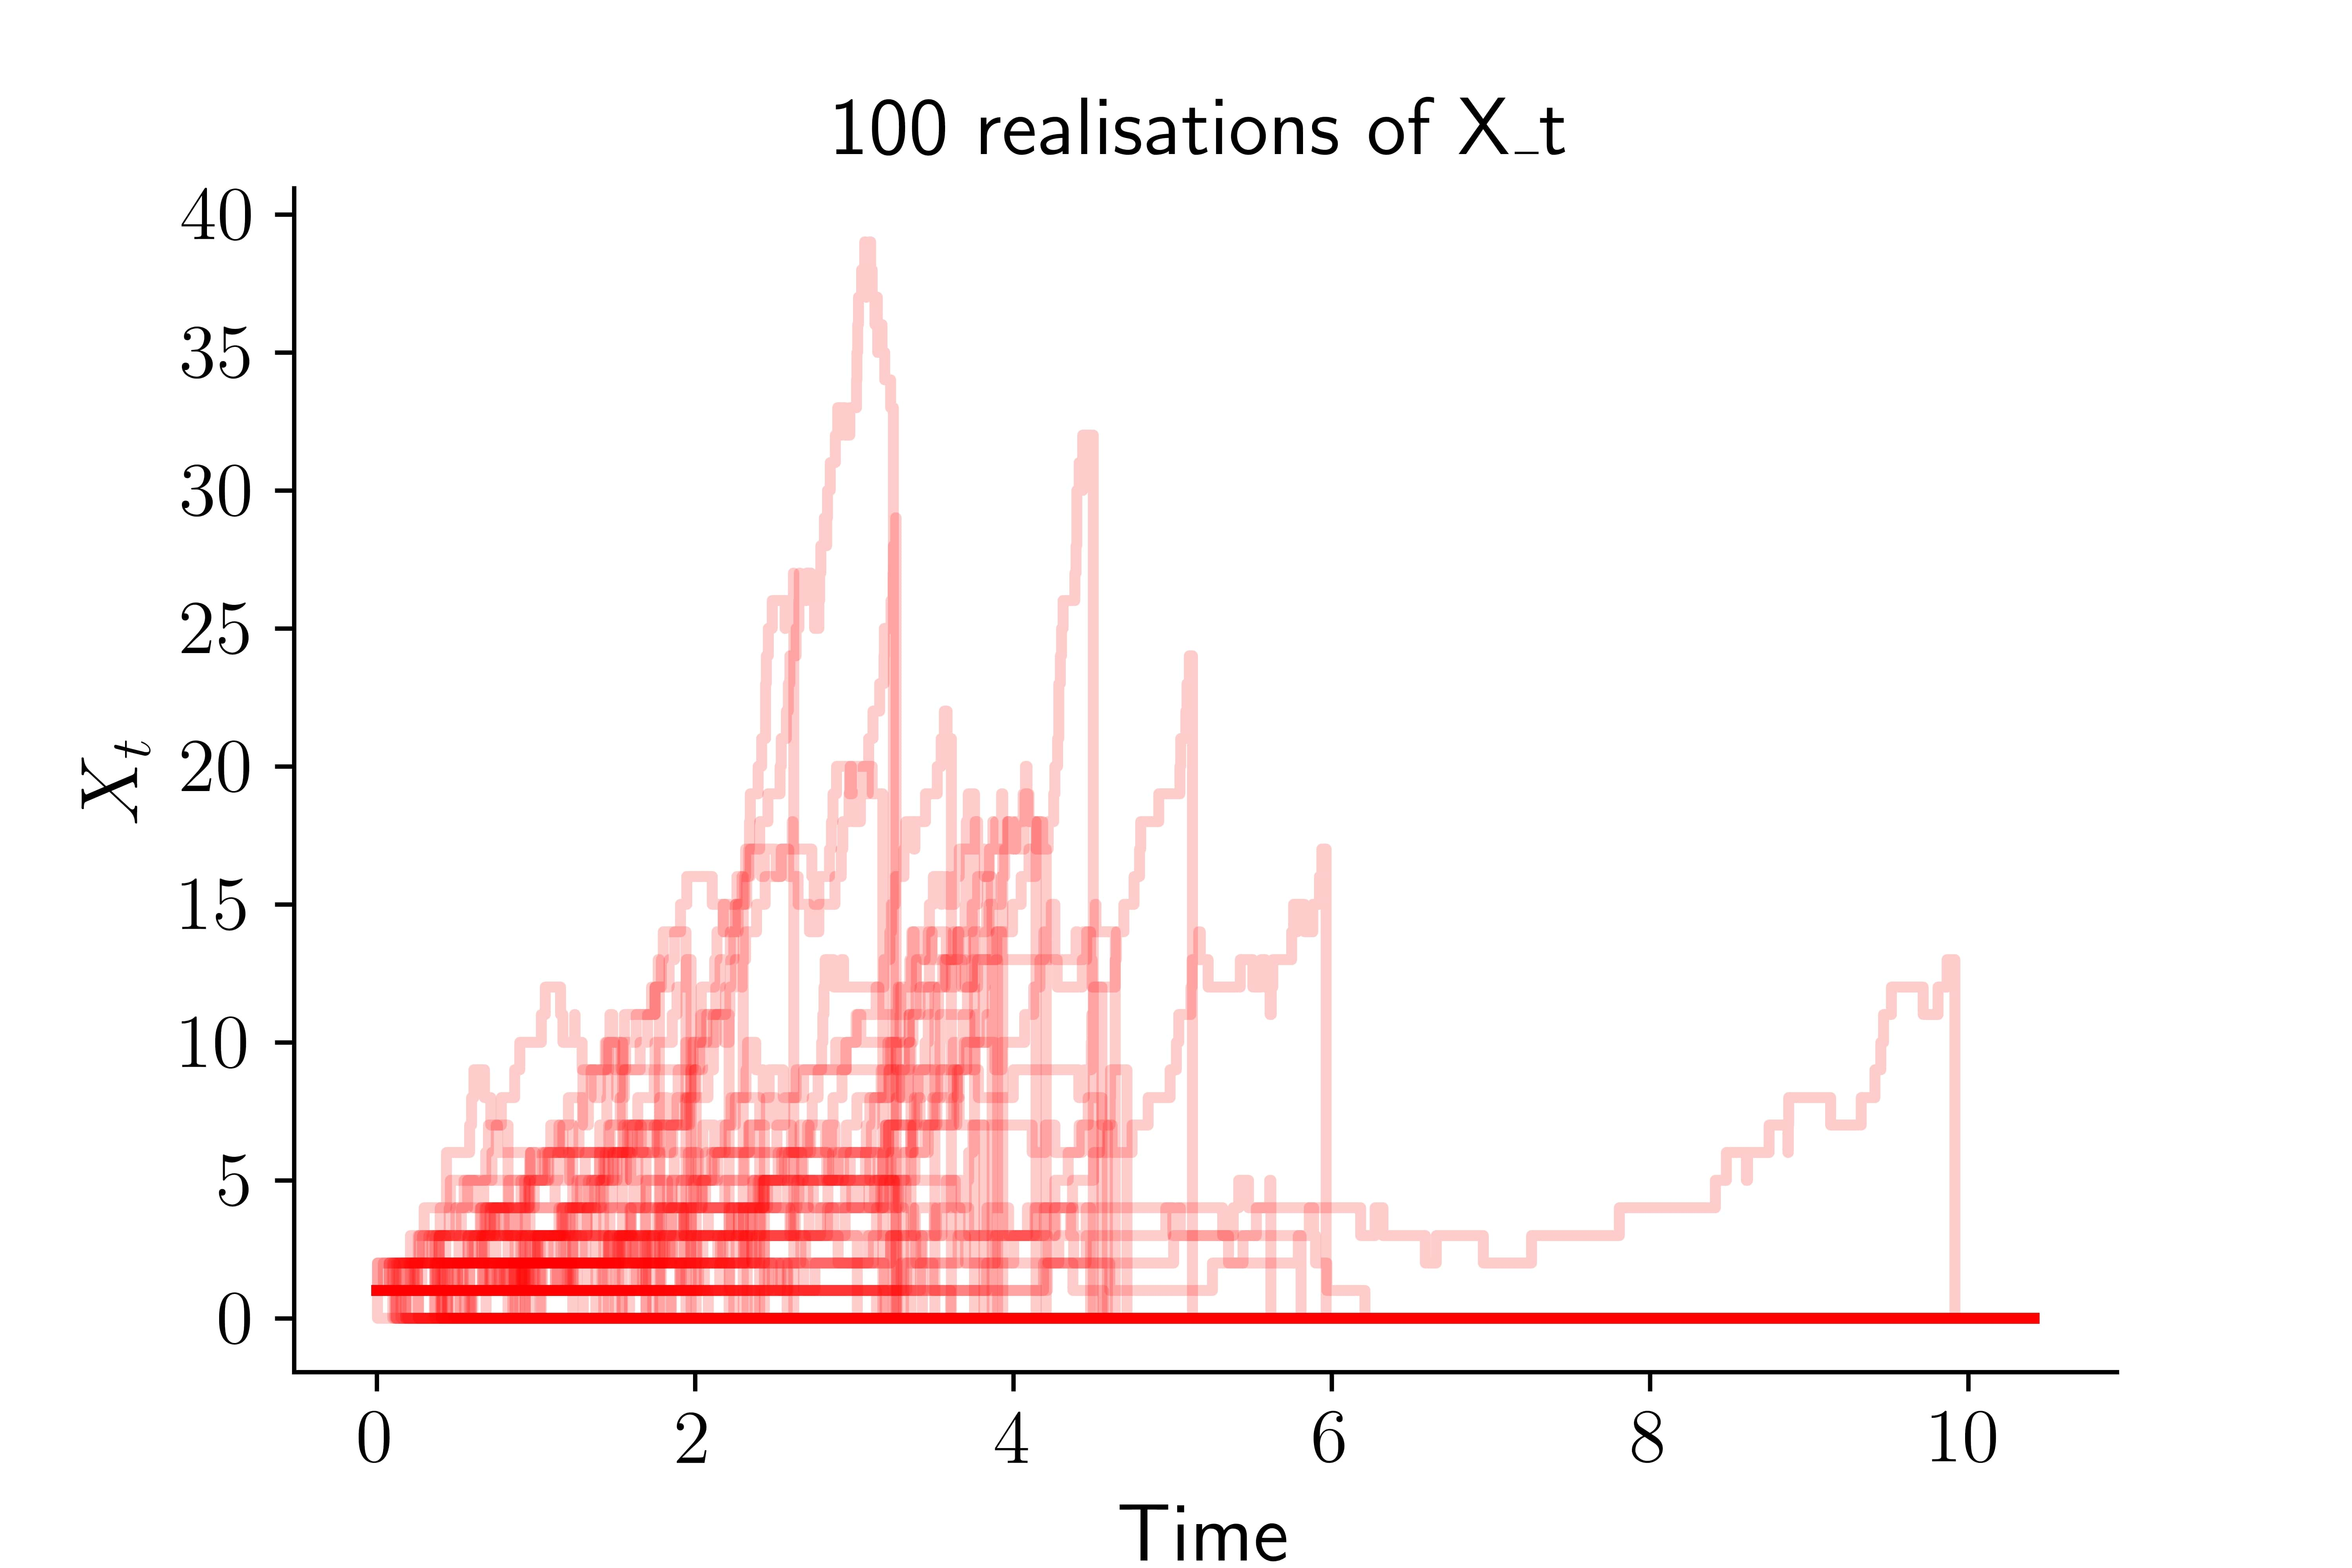
\includegraphics[width = 0.7\textwidth]{figures/BDRsimulations.jpg}
\caption{100 realisations of $\xt$ generated using the Gillespie algorithm. $\lambda = 1$, $\mu = 0$, $\delta = 0.1$. }
\label{fig:BDRsimsX}
\end{figure}

Sample paths of the process are shown in \Figref{fig:BDRsimsX}: realisations
rise and fall stochastically, some collapsing to the absorbing state $0$, others
terminating abruptly at catastrophe.

\figureflag{F3.6}{Gillespie simulations re-rendered}{%
\textbf{Purpose:} the two existing Gillespie simulation figures
(\Figref{fig:BDRsimsX}, \Figref{fig:BDRsimsW}) were produced early in the work
as jpg screenshots; re-rendering them in the unified Python style brings them
to thesis standard without changing their content. \textbf{Type:} Python
simulation (Gillespie algorithm), upgrade of the two existing jpgs, which
remain in place until the re-rendered versions exist. \textbf{Content:} 100
realisations of $X_t$ (panel 1) and of $W_t$ (panel 2), parameters
$(\lambda,\mu,\delta)=(1,0,0.1)$, $X_0=1$, identical to the existing figures;
each realisation a step function on $t\in[0,20]$; realisations of $X_t$ end at
$0$ or jump to the catastrophe state $H$; realisations of $W_t$ jump from $0$
to $X_{\tau^-}$ at the burst time $\tau$ and hold. \textbf{Axes:} $t$
(horizontal, 0 to 20), count (vertical); no legend required for the
realisations themselves; annotate one representative burst in panel 2.
\textbf{Style:} unified Python style --- default matplotlib with \texttt{tab:}
colours, grid alpha 0.25, \texttt{tight\_layout}, PDF output, fonts matching
the chapter. \textbf{Data source:} Gillespie exact simulation: from state
$n\ge1$ draw the next event among birth ($\lambda n$), death ($\mu n$),
catastrophe ($\delta n$) with exponentially distributed waiting time of rate
$(\lambda+\mu+\delta)n$; state $0$ is absorbing and catastrophe moves the pair
to $(H, W=n)$. \textbf{Placement:} replace the two jpg figures in
\Secref{sec:process_definition} when generated.}

\subsection{Choice of rupture state}

An alternative definition lists the ``catastrophe state'' as $0$ instead of a
separate state $H$, and it would make some intuitive sense to arrange the
process like this. After all, following rupture of an infected cell, there are
subsequently $0$ replicative units within it --- but then, the cell also no
longer exists. Ultimately, whether we ascribe the catastrophe state to $0$ or
$H$ is of no material significance to the dynamics: the burst times and sizes
observed are unchanged. But a distinction is created in some of the formulas.
These will be mentioned as we continue; for our purposes, the catastrophe
transition is taken to the isolated state $H$.

\figureflag{F3.2}{Rupture conventions: killing versus catastrophe}{%
\textbf{Purpose:} fix, once and for all, the convention distinction between the
``killing'' convention (rupture returns the process to state $0$) and the
``catastrophe'' convention (rupture moves it to a separate absorbing state
$H$), which is used throughout the thesis and on which the definition of
$\Ifix(t)$ depends. \textbf{Type:} TikZ schematic, two panels side by side.
\textbf{Content:} left panel ``killing'': states $0,1,2,\ldots$ with arrows
$n\to n+1$ ($\lambda n$), $n\to n-1$ ($\mu n$), and catastrophe arrows from
each $n\ge1$ landing back in state $0$, labelled $\delta n$; right panel
``catastrophe'': the same chain plus a separate absorbing state $H$ receiving
the $\delta n$ arrows. In each panel draw one representative sample path: in
the killing panel the path ends indistinguishably among the deaths at $0$; in
the catastrophe panel the path ends at $H$. \textbf{Labels:} panel titles
``killing'' and ``catastrophe''; state and rate labels as in F3.1.
\textbf{Style:} TikZ, inline with chapter fonts, matching F3.1.
\textbf{Placement:} the ``Choice of rupture state'' subsection of
\Secref{sec:process_definition}.}

\subsection{Post-catastrophe count}

In the context we are considering, the catastrophe signifies the rupture of an
infected cell, and following this release some count of infectious units enters
the extracellular medium. This post-rupture count, assuming no further
dynamics, is fixed by the final value of $\xt$ prior to catastrophe, and it
remains at that value for all future time. We refer to this post-rupture count
as $\wt$, itself a stochastic process: $\wt = 0$ for $t<\tau$, and
$\wt = \xx_{\tau^-}$ thereafter for $t \ge \tau$, where $\tau$ is the time of
cell rupture. The process $\wt$ is included in the definition as follows, to
describe the full stochastic process $(\xt, \wt)$:
\begin{align*}
\pr{\Delta \xt = 1, \Delta \wt = 0} &= \lambda \xt \cdot \delt&&\text{(birth)}\\
\pr{\Delta \xt = -1, \Delta \wt = 0} &= \mu \xt  \cdot \delt&&\text{(death)}\\
\pr{\Delta \xt = 0, \Delta \wt = 0} &=1 -  (\lambda+\mu+\delta) \xt  \cdot \delt&&\text{(no event)}\\
\pr{\xx_{t+\Delta t} = H, \ww_{t+\Delta t} = \xx_t} &=\delta \xt  \cdot \delt&&\text{(catastrophe)}
\end{align*}
(using the shorthand $\Delta \xt = \xx_{t+\Delta t}  -  \xt$).

\begin{figure}[H]
\centering
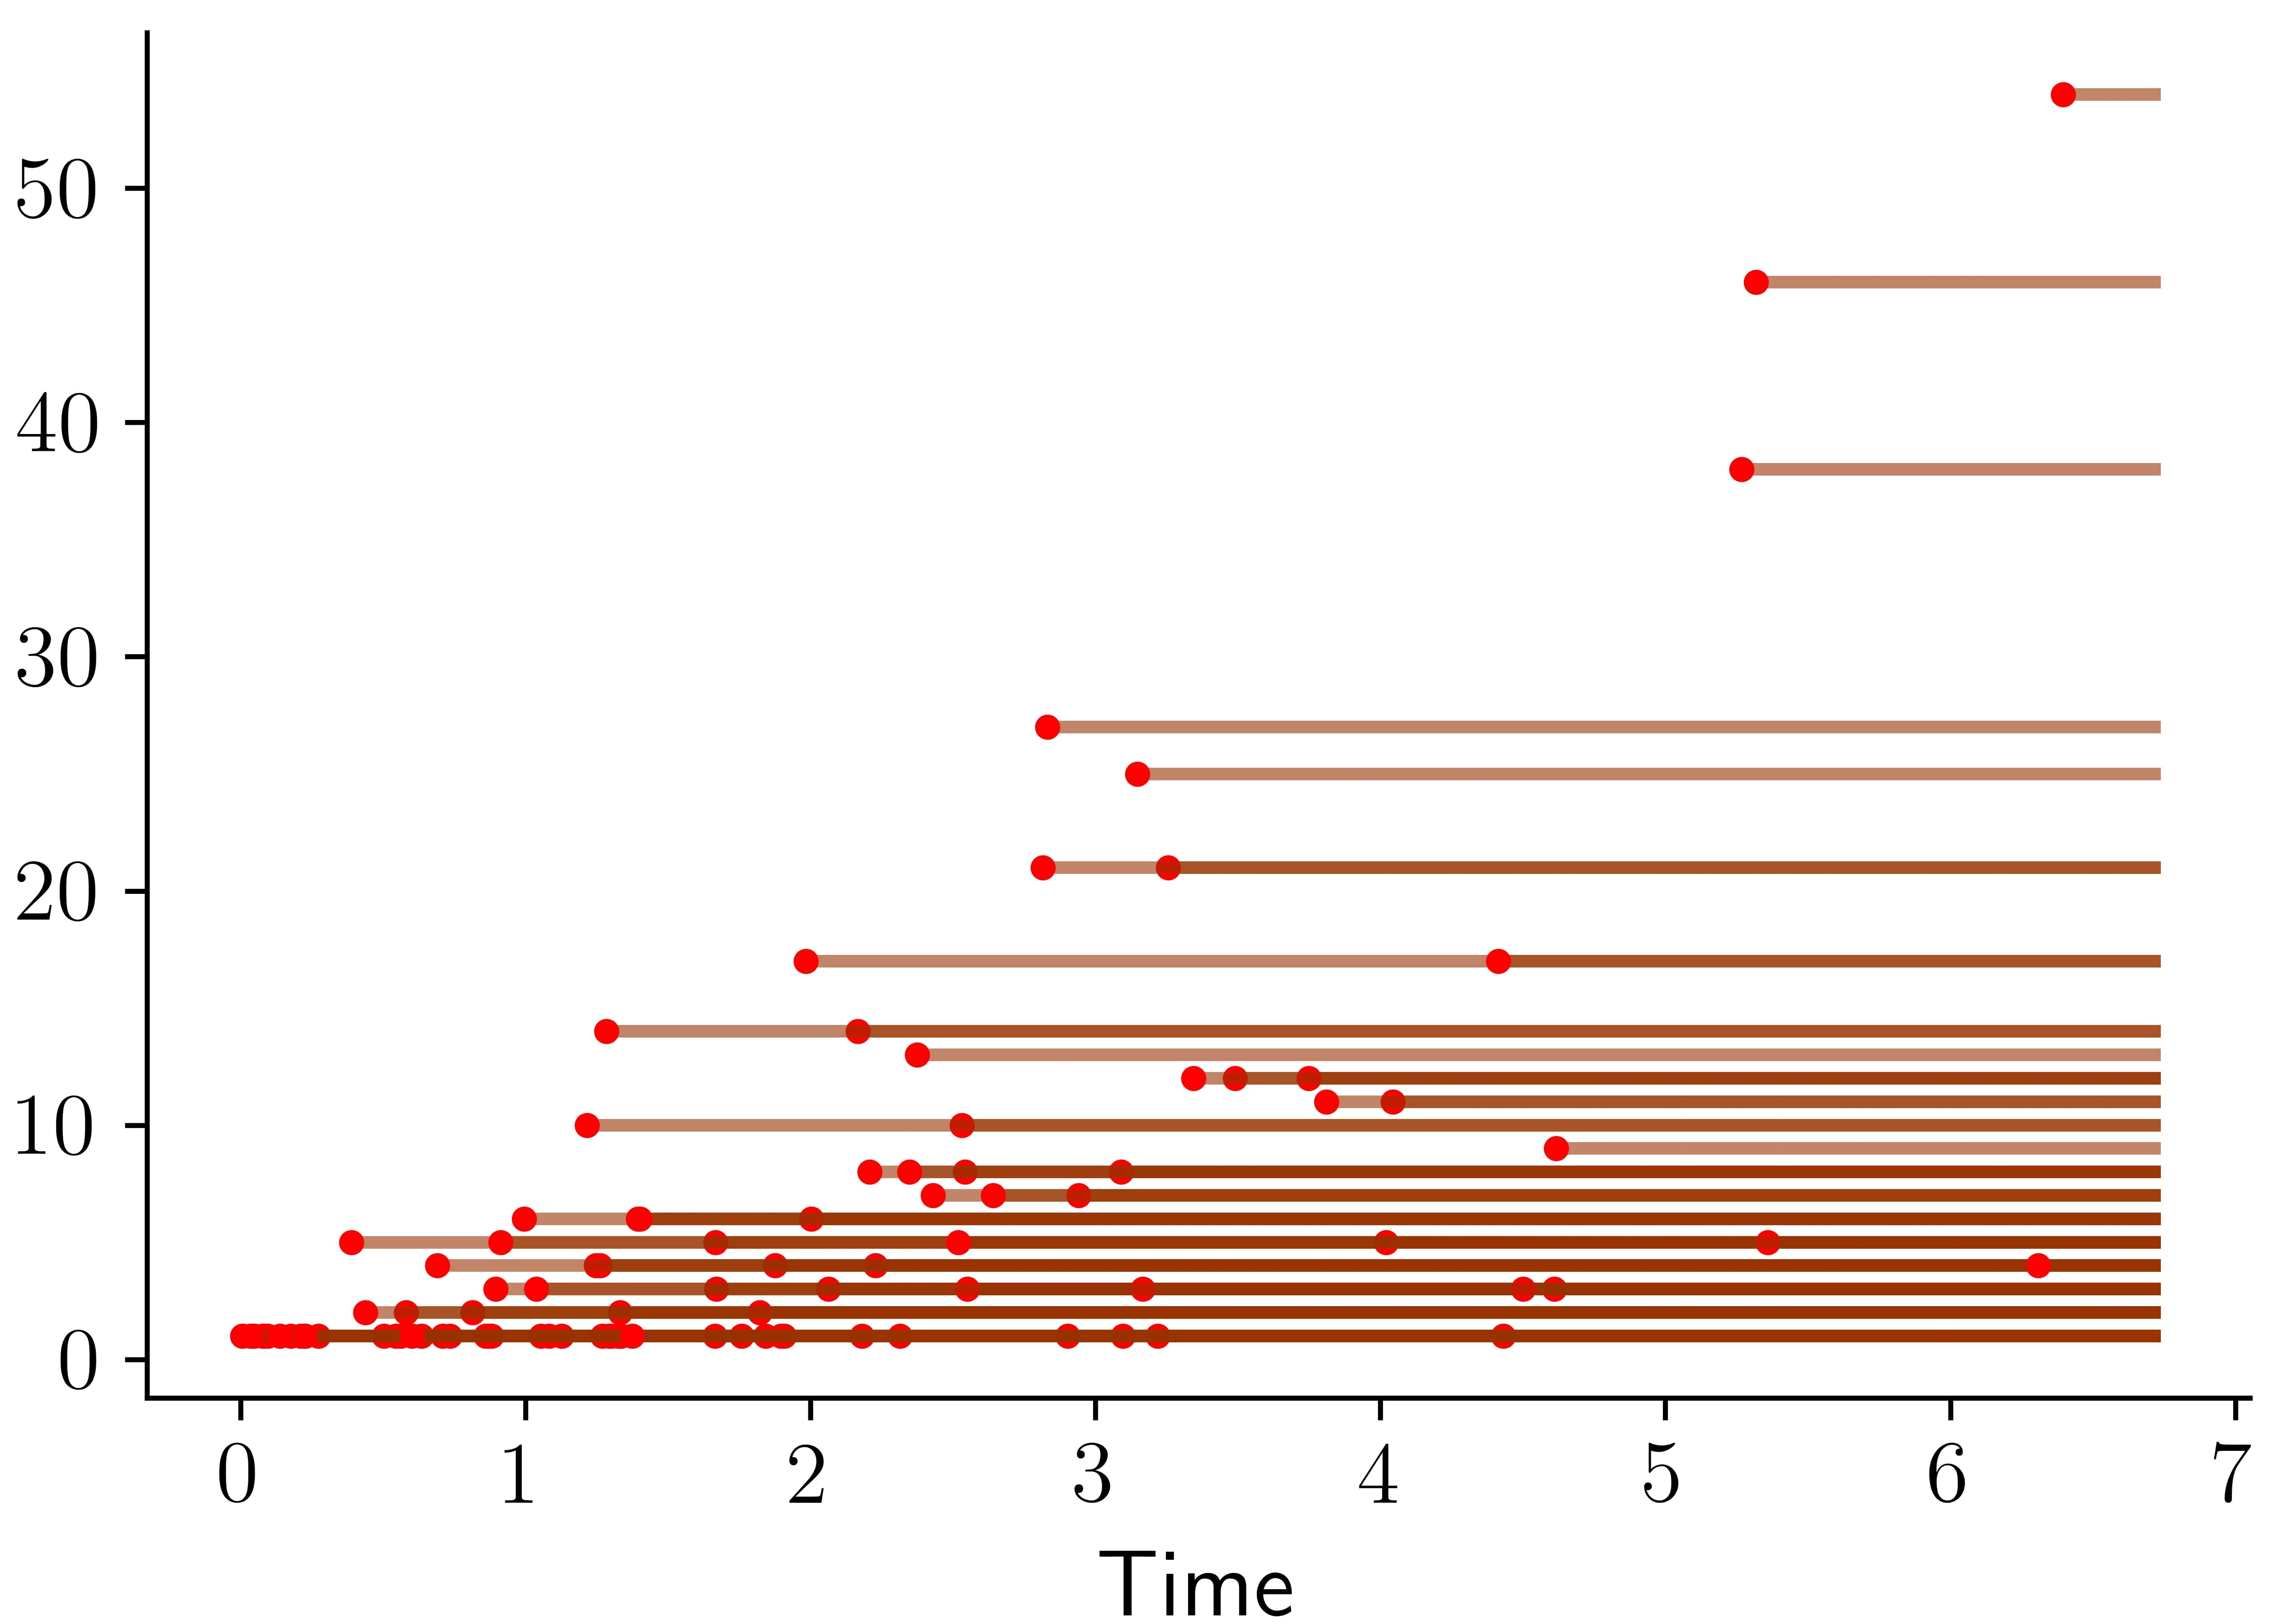
\includegraphics[width = 0.55\textwidth]{figures/BDRsimulationsY2.jpg}
\caption{100 realisations of $\wt$ generated using the Gillespie algorithm. $\lambda = 1$, $\mu = 0$, $\delta = 0.1$. }
\label{fig:BDRsimsW}
\end{figure}

\Figref{fig:BDRsimsW} shows the corresponding released-count realisations: each
path holds at zero until its cell ruptures, then jumps to the intracellular
load accumulated at that instant and stays there. The pair $(\xt,\wt)$ is the
object this chapter dissects, and the two components will be studied through
their expectations, variances, and eventually their full distributions.
